\documentclass[conference]{IEEEtran}

% Use of outside images
\usepackage{graphicx} 
% Use text inside euqations
\usepackage{amsmath}

%\usepackage{balance}
\usepackage{float}
\floatstyle{plaintop}
\restylefloat{table}

% Correct bad hyphenation here
\hyphenation{op-tical net-works semi-conduc-tor}

% Begin the paper here
\begin{document}

% Paper title
% Can use linebreaks \\ within to get better formatting as desired
\title{API Evolution: A Study of Software Stability and Change Trends}

% Authors names
\author{\IEEEauthorblockN{Jordan Ell}
\IEEEauthorblockA{University of Victoria\\
British Columbia, Canada \\ jell@uvic.ca}
\and
\IEEEauthorblockN{Braden Simpson}
\IEEEauthorblockA{University of Victoria\\
British Columbia, Canada \\ braden@uvic.ca}
\and
\IEEEauthorblockN{Daniela Damian}
\IEEEauthorblockA{University of Victoria\\
British Columbia, Canada \\ danielad@csc.uvic.ca}
}

% Make the title area
\maketitle

\begin{abstract}
Something
\end{abstract}

\section{Introduction}
Intorduction goes here.

\section{Related Work}
Related work goes here.

\section{Methodology}
In order to answer our research question, we decided to use the tool ChangeDistiller created by Fluri et al.~\cite{}. This tool allows us to detect fine grained
source code changes in Java projects This tool works by building an abstract syntax tree of a file before and after a code change, then it tries to determine
the smallest possible edit distance between the tree. This results in the source code change at a fine grained level performed in the commit.

We took ChangeDistiller and applied it across 10 open source Java projects. For each of the projects, we obtained the software configuration management (SCM) system
which is used to store all source code changes of a project. When it was necessary, we converted some forms of SCM system to Git in order to reduce implementation
burdens of using multiple SCMs. Once the SCM was obtained, we used ChangeDistiller and iterated over every commit found in a project's git master branch. We stored
34 of ChangeDistiller's built in source code change types for each commit. We noted how many of each change type was performed in each commit and stored that information
in a PostgreSQL database. In order to filter and protect our results, we manually inspected the 10 Java projects studied in order to identify code built for test.
We separated changes to this test code from all other code to ensure our results only focused on real implementation while allowing us to study changes to
test based code separately.

Once the ChangeDistiller information was collected, we decided to examine software change trends surrounding releases of the project's we had selected. Since releases
have preconceived notions of software stability, we decided that by studying the types of changes surrounding these releases, we could get a better understanding of
what types of source code changes or trends constitute software stability or maturity. In order to study the release points, we went to each of our 10 project's 
home pages on-line and looked through their release histories for major, minor, alpha, beta, and release candidate type releases. In total we identified 472 releases
across our 10 studied projects.  

Once the release dates were collected we set about analyzing out data by creating average change ratios surrounding the release dates of each 
project as a way to measure the trend of a particular change type at a release type. 
To do this we used Equation~\ref{eq:norm}. Equation~\ref{eq:norm} works to create a change ratio by first creating a numerator by summing across all releases of
a given release type a sum of a particular change type in commits ($T_c$)
from the release date ($r$) to a given number of days after the release ($d$) divided by the number of commits in this date range ($|c|$). Next the denominator
is created by summing across all release of a given release type
a sum of that same particular change type in commits($T_c$) from a given number of days ($d$) before the release date ($r$) to
the release date divided by divided by the number of commits in this date range ($|c|$). This numerator and denominator form the final change ratio.
This equation gives us a ratio of a particular change type happening before and after a particular release. If the ratio is above 1 then that particular change
type occurs more frequently after the release and if it is below 1 then is occurs more frequently before the release. For the purposes of our study, we set the
number of days before and after the release ($d$) to 60 as the projects studies had many months in between their major releases. This quantitative data
formed much of the basis for the results to come in Section~\ref{sec:results}

\begin{equation}
\text{ChangeRatio} = \frac{ \sum_{r_0}^{r_n}\sum_{c=r}^{r+d} T_c / |c|} { \sum_{r_0}\sum_{c=r}^{r-d} T_c / |c|}
\label{eq:norm}
\end{equation}

Aside from generating quantitative data, we also created a web application for the visualization of the data called API Evolution (APIE). This visualizer allowed
us to inspect a single project and a single change type metric at a time (see Figure~\ref{fig:apie}) for qualitative analysis of software evolution trends. We
used this tool to manually inspect 4 specific change type trends surround release dates. To do this, we aggregated change types across 50 commits, meaning that
each point in the graph represented the date of a commit and the sum of the particular change type's occurrences over the last 50 commits. This was used to smooth
out the curves presented by the tool to allow easier manual inspection. Manual inspections were labeled into 4 categories: upward trending, local maximum, downward
trending, and local minimum. Since the graphs were quite turbulent, best estimations were given by two judges at each release point to fit the graph into the aforementioned
4 slope categories. The two judges used 1.5 months before and after the release date as start and end points for the graph trend line.

% APIE graph figure
\begin{figure}[tb!]
\centering
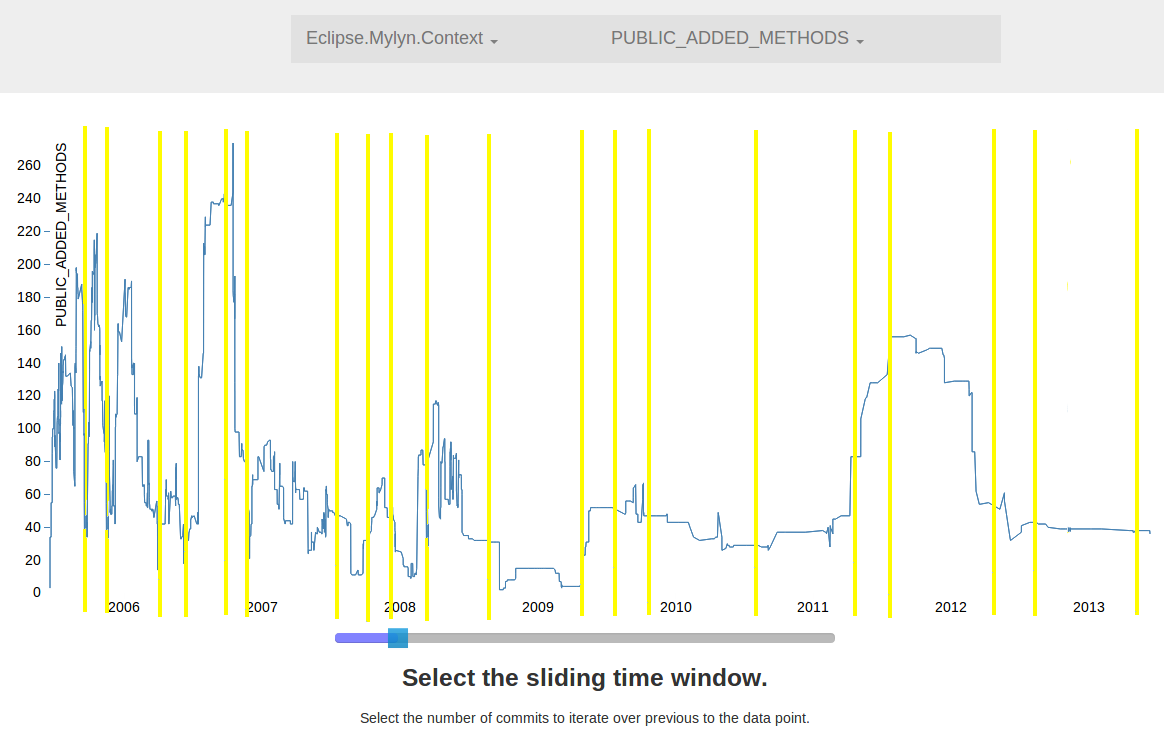
\includegraphics[width=0.5\textwidth]{images/apie.png}
\caption{An screen shot of the APIE visualizer showing project Eclipse.Mylyn.Context with change type PUBLIC\_ADDED\_METHODS being analyzed.\label{fig:apie}}
\end{figure}

We performed 1888 manual inspections across 10 projects, 472 release dates and 4 change types, and used this data to form the basis of our qualitative data.
Quantitative data was cross validated with qualitative data to form some of the final results to be seen in the next section. 

\section{Results}
\label{sec:results}

To answer our research question, we conducted a case study of 10 open source Java projects. These projects are: eclipse.jdt.core, eclipse.jdt.ui, eclipse.jetty.project, 
eclipse.mylyn.commons, eclipse.mylyn.context, hibernate-orm, hibernate-ogm, hibernate-search, eclipse.maven.core, and eclipse.maven.surefire. These project were chosen
because of their high use amongst other Java projects and to study specific ecosystems of projects and their evolution trends.

Due to the space requirements of this paper, we focus our results on Major releases of the 10 case study projects and a select few of the calculated change ratios. 
There were 109 major releases across the 10 studied projects. All of the major findings as per values computed from Equation~\ref{eq:norm}
can be seen in Table~\ref{tab:ratio}.

\begin{table}[h]
\begin{center}
\begin{tabular}{| l | c | c | c |}
\hline
Object & Added & Changed & Removed\\
\hline
Public Classes & 0.78 & 0.76 & 0.67 \\
Public Methods (Signature) & 1.12 & 0.66 & 2.45 \\
Public Methods (Bodies) & - & 0.86 & - \\
Private Classes & 0.59 & 0.92 & 0.32 \\
Private Methods (Signatures) & 0.86 & 0.91 & 1.49 \\
Private Methods (Bodies) & - & 0.91 & - \\
\hline
\end{tabular}
\end{center}
\caption{Implementation oriented change types and their normalized average change ratios at 60 days on each side of releases. \label{tab:ratio}}
\end{table}

As it can be seen in Table~\ref{tab:ratio}, there a few notable change type trends around major releases. We can see that any changes to public classes are
more likely to occur before a major release than after, noting that the addition, changing, and deletion of public classes have change ratios of 0.78, 
0.76 and 0.67 respectively. The two most drastic change type trends to note from this table however are the removing of public methods and the removing
of private classes. We can see that public methods are more than twice as likely to occur after a major release than before it and the removal of 
private classes is three times as likely to happen before a major release than after. 

In terms of added code, we found as per Table~\ref{tab:ratio} that additions to private classes are a large indicator of a project being at a stable
release point with almost being twice as likely to occur before a major release than after. A large surprise to changed code indicators was that of the
public method bodies. We can see that with a change ration of 0.86 there is not a major indication of these types of changes happening before or after a 
release which leads us to believe that method implementation may not be able to be detected as stable through software metrics. Changes
to method signatures also point towards changes before a release rather than after which may indicate that stable software only needs to be stable after the
release and not prior, as changing method signature is considered a fairly unstable change~\cite{Fluri}.

Our qualitative results from manual graph inspections can be seen in Table~\ref{tab:qual}. These results show that adding, changing signatures and bodies of, and
removing public methods tend to all be at a local minimum of change type trends at major releases.

\begin{table}[h]
\begin{center}
\begin{tabular}{| l | c | c | c | c |}
\hline
Change Type & Upward Trend & Local Maximum & Downward Trend & Local Minimum\\
\hline
Added Public Methods & 21.6\% & 17.2\% & 14.7\% & 33.6\% \\
Changed Public Methods (Signature) & 6.0\% & 19.8\% & 19.0\% & 39.7\% \\
Changed Public Methods (Bodies) & 9.2\% & 16.5\% & 26.6\% & 37.6\% \\
Removed Public Methods & 7.8\% & 16.4\% & 12.9\% & 41.4\% \\
\hline
\end{tabular}
\end{center}
\caption{Qualitative graph analysis results. \label{tab:qual}}
\end{table}

Lastly we found that software changes related to testing can be highly used as an indicator of a major release point within the projects studied. The change
ratios found can be seen in Table~\ref{tab:test}. As it can be seen, the three largest indicators of a project release and stability with regards to test based
changes as the addition of test classes, the removal of test classes, and the removal of test methods.

We summarize our key findings as to source code change type trends which can be found at points of stability as the following: the addition of private classes more often
before a stable point, the changing of public method signatures more often before a stable point, the removal of public methods more than twice as often
after a stable point, the removal of private classes three times as often after a stable point, and the removal of test classes more than twice as often after
a stable point. There are of course other change ratios to consider as listed in this section, however we found the aforementioned to be the most indicative of 
software stability around major releases.

\begin{table}[h]
\begin{center}
\begin{tabular}{| l | c | c | c |}
\hline
Object & Added & Changed & Removed\\
\hline
Classes & 0.72 & 0.86 & 0.36 \\
Methods & 1.55 & 0.98 & 1.93 \\
\hline
\end{tabular}
\end{center}
\caption{Test oriented change types and their normalized average change ratios at 60 days on each side of releases. \label{tab:test}}
\end{table}

\section{Future Work}

\section{Conclusions}

Software stability is an often used measure in determining some aspects of code quality. This paper has present some initial indications as to how
software stability may be found, based on major release stabilities, by analyzing source code change type trends both before and after major software
releases. The source code change trends found in this paper, in combination with future work and analysis, will allow for the detection of stable code
points throughout a software projects life time. This paper has also shown the beginnings of a visualization for source code change trends which may
be used as a visual cue towards project stability and potential areas of instability where action may need to be taken.

% End of the paper
\end{document}

\bibliographystyle{IEEEtran}
%\balance
\bibliography{paper}
